\documentclass[a4paper, twocolumn]{article}

% Packages
\usepackage[utf8]{inputenc}
\usepackage{graphicx}
\usepackage{hyperref}
\usepackage{amsmath}
\usepackage{amsfonts}
\usepackage{amssymb}
\usepackage[left=2cm,right=2cm,top=2cm,bottom=2cm]{geometry}
\usepackage{fancyhdr}
\usepackage{glossaries}
\usepackage{listings}
\usepackage{xcolor} % Extended color functionalities
\usepackage{graphicx} % Required for inserting images
\usepackage{tikz}
\usetikzlibrary{automata, positioning, arrows}
\usepackage{float}
\usepackage{subcaption}


\hypersetup{colorlinks=true, linkcolor=blue}

% Define custom colors
\definecolor{codegreen}{rgb}{0,0.6,0}
\definecolor{codegray}{rgb}{0.5,0.5,0.5}
\definecolor{codepurple}{rgb}{0.58,0,0.82}
\definecolor{backcolour}{rgb}{0.95,0.95,0.92}

% MATLAB style for highlighting
\lstdefinestyle{mystyle}{
    backgroundcolor=\color{backcolour},   
    commentstyle=\color{codegreen},
    keywordstyle=\color{magenta},
    numberstyle=\tiny\color{codegray},
    stringstyle=\color{codepurple},
    basicstyle=\ttfamily\footnotesize,
    breakatwhitespace=false,         
    breaklines=true,                 
    captionpos=b,                    
    keepspaces=true,                 
    numbers=left,                    
    numbersep=5pt,                  
    showspaces=false,                
    showstringspaces=false,
    showtabs=false,                  
    tabsize=2
}

\lstset{style=mystyle}

% Glossary entries
\newacronym{pep}{PEP}{Peak Envelope Power}
\newacronym{papr}{PAPR}{Peak to Average Power Ratio}
\newacronym{ofdm}{OFDM}{Orthogonal Frequency Division Multiplexing}

% Document
\begin{document}

\begin{titlepage}
    \begin{center}
        \vspace*{1cm}

        \Huge
        \textbf{Modulation Waveforms Lab Report}

        \vspace{0.5cm}
        \LARGE
        EXPERIMENT CP-SRP
        EE20017
        
        \vspace{1.5cm}

        \textbf{Jake Stewart}\\
        \textbf{JS3910}\\

        \textbf{Eugene Levinson}\\
        \textbf{EL769}\\
        \vspace{0.8cm}

                \vfill
                
\includegraphics[width=0.5\textwidth]{university_logo.png}

                \Large
                Electrical and Electronic Engineering\\
                University of Bath\\
                United Kingdom\\
                \today
                

            \end{center}
        \end{titlepage}

        \newpage
        \tableofcontents

        \section{Introduction}
        This report presents the findings from the "Modulation Waveforms" lab, part of the EE20017 Communication Principles module. The primary objective was to explore AM modulation and its signal processing intricacies utilizing Matlab for practical experiments.
        
        \section{Modulation Tests}
        Utilizing the AM\_2.m script, square and triangle waves were modulated by adjusting modulation parameters including amplitude, frequency, and phase to align with predefined specifications. Adjustments were also made to load resistance and loss parameters as required. The script generates insightful plots for signal analysis, which, combined with additional calculations integrated into the Matlab scripts, facilitated a thorough examination of \gls{pep} and \gls{papr}.
        
        \begin{lstlisting}[language=Matlab, caption={Signal processing calculations}, label={lst:singnalcalcs}]
        % AM Power
        R = 50; % Ohms
        Power = (Signal.^2) / (2*R); % RMS Power in Watts V^2/2R
        % Peak Envelope Power
        PEP = max(Power)
        % Peak to Average Power Ratio
        PAPR = PEP/mean(Power)
        \end{lstlisting}

        \subsection{Results}
        \subsection*{Square Wave Modulation Analysis}
        The modulation of a carrier signal with a square wave was conducted using the script and parameters provided. The process involved adjusting the modulation parameters to achieve the desired waveform and analyzing the outcome using MATLAB for signal processing calculations.
        
        To compute the Peak Envelope Power (\gls{pep}), the formula $PEP = \frac{(V_{peak}/\sqrt{2})^2}{R}$ was employed, where $V_{peak}$ denotes the maximum amplitude of the waveform. This calculation was facilitated by MATLAB, performing an element-wise operation to determine the power for each sample point in the modulated signal and identifying the maximum value.
        
        The mean power, \(P_{\text{mean}}\), was calculated using the formula: 
        \[P_{\text{mean}} = \frac{V_c^2}{2R} + \sum_{i=1}^{n} \frac{V_{m_i}^2}{2R}\]
        where \(V_c\) represents the RMS voltage of the carrier signal, \(V_{m_i}\) the RMS voltage of each modulation signal, \(R\) the load resistance, and \(n\) the number of modulation frequencies. The Peak to Average Power Ratio (\gls{papr}) was then determined as $PAPR = \frac{PEP}{P_{mean}}$.
        
        The results for the square wave modulation were as follows:
        \begin{itemize}
            \item $PEP$: 214.7 mW
            \item $P_{mean}$: 45.4 mW
            \item $PAPR$: 4.7312
        \end{itemize}
            
        \begin{figure}[H]
            \centering
            \begin{subfigure}{0.45\textwidth}
                \centering
                \includegraphics[width=\textwidth]{Images/AM_RX_1/Square Wave/AM Spectrum.jpg}
                \caption{AM Spectrum of square modulated signal}
                \label{fig:amspectrum-square}
            \end{subfigure}
            \hfill
            \begin{subfigure}{0.45\textwidth}
                \centering
                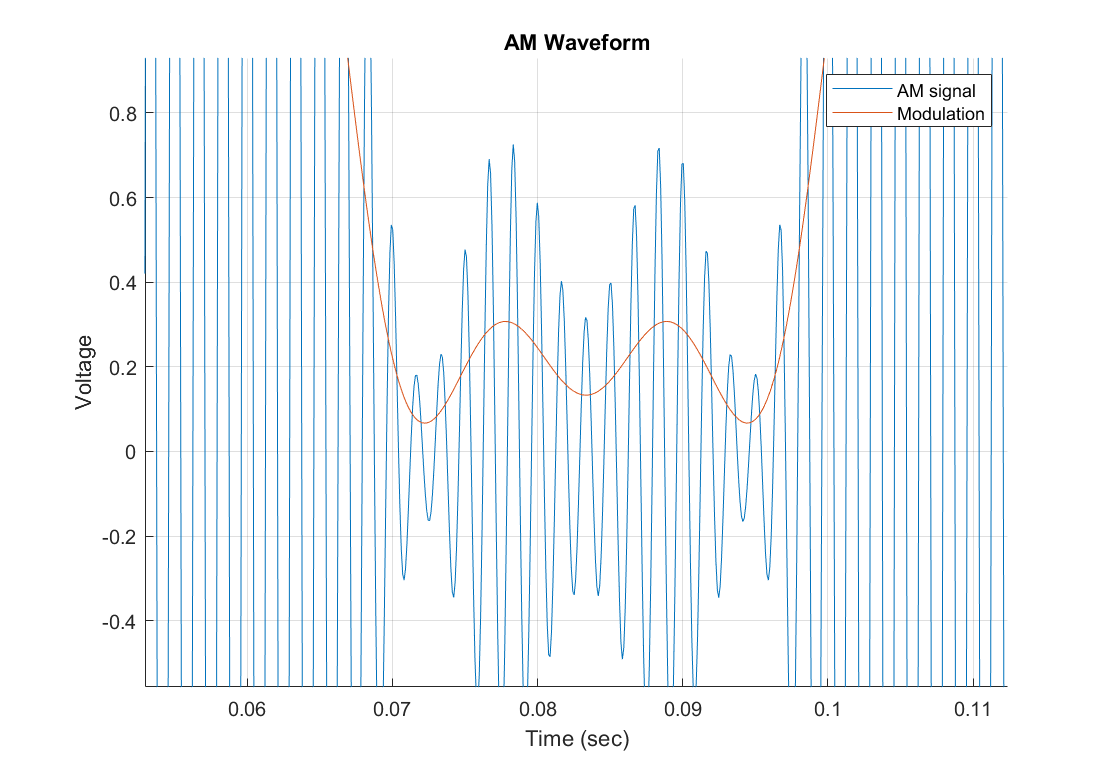
\includegraphics[width=\textwidth]{Images/AM_RX_1/Square Wave/No Distortion.png}
                \caption{Modulation signal indicating no distortion}
                \label{fig:nodistortion-square}
            \end{subfigure}
            \caption{Analysis of square wave modulation}
        \end{figure}

        An analysis of the AM spectrum revealed the following power distribution in mW for the carrier and modulation frequencies: $14.4000$, $3.6000$, $0.3992$, $0.1440$ for $f_c$, $f_{m1}$, $f_{m2}$, $f_{m3}$, respectively. The sidebands accounted for 28.47\% of the total power. The inspection confirmed that the modulation process introduced no distortion, as evidenced by a clean FFT plot and the absence of unintended harmonics.

        
        \subsection*{Triangular Wave Modulation Analysis}
        In this experiment, the modulation signal's parameters were fine-tuned as per the laboratory instructions to closely replicate a triangular waveform. The methodology for calculating the Peak Envelope Power (\gls{pep}) and the Peak to Average Power Ratio (\gls{papr}) mirrored the approach utilized for the square wave modulation, leading to the following findings:
        
        \begin{itemize}
            \item $PEP$: 369.6 mW
            \item $PAPR$: 8.14
        \end{itemize}

        \begin{figure}[H]
            \centering
            \begin{subfigure}{0.45\textwidth}
                \centering
                \includegraphics[width=\textwidth]{Images/AM_RX_1/Triangular Wave/AM Spectrum.jpg}
                \caption{AM spectrum of triangular modulated signal}
                \label{fig:amspectrum-triangle}
            \end{subfigure}
            \hfill
            \begin{subfigure}{0.45\textwidth}
                \centering
                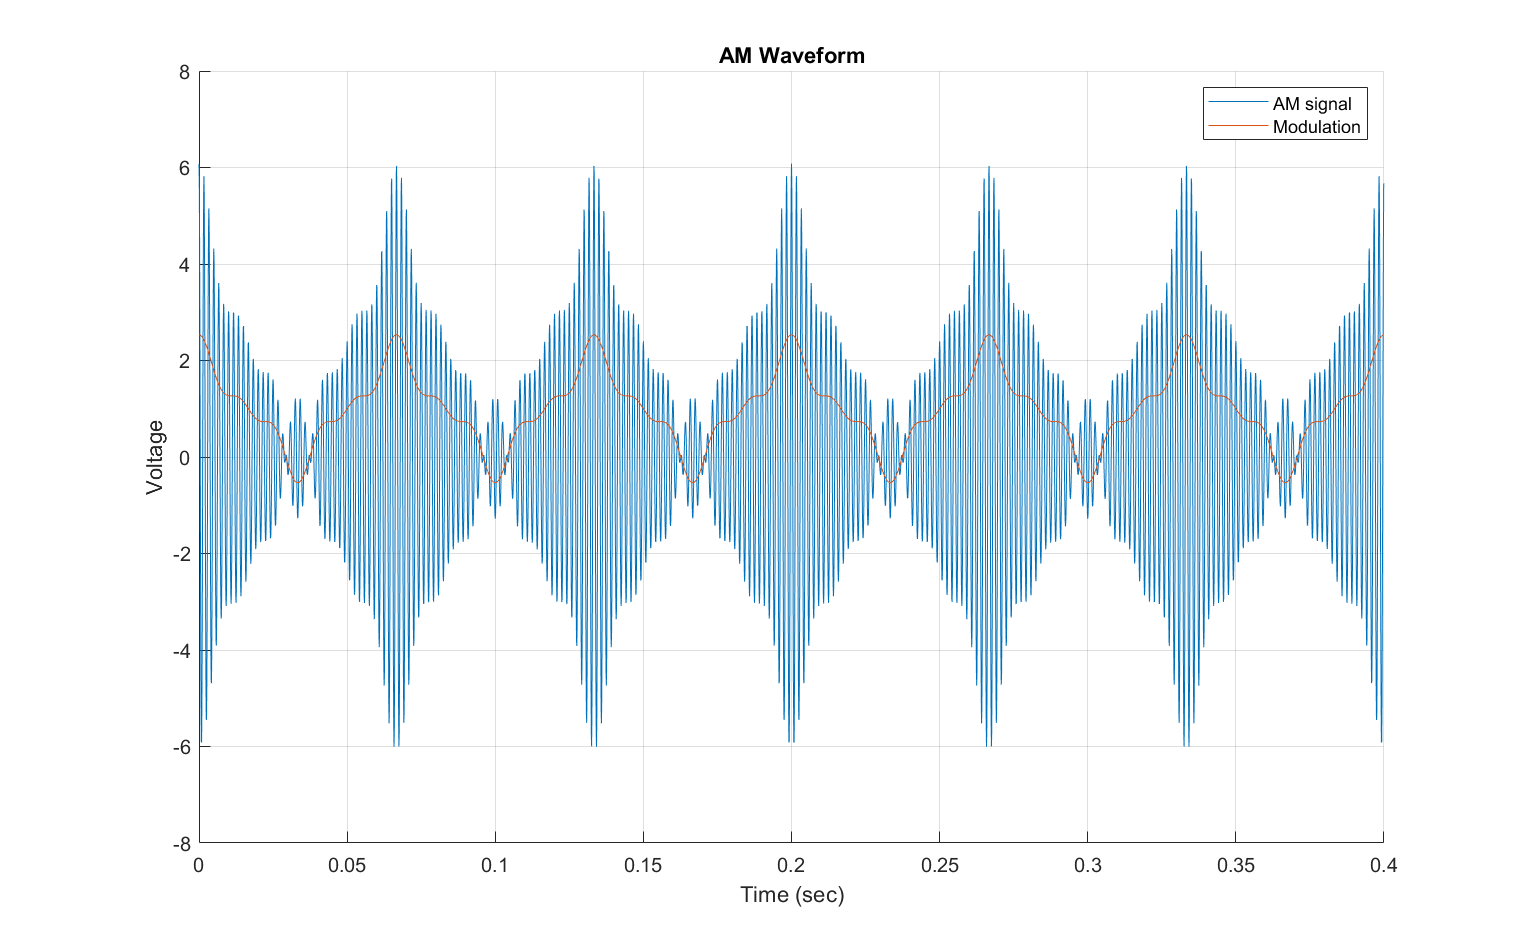
\includegraphics[width=\textwidth]{Images/AM_RX_1/Triangular Wave/Full AM.png}
                \caption{Overall view of AM and triangular modulation signal}
                \label{fig:fullam-triangle}
            \end{subfigure}
            \caption{Spectral and signal analysis of triangular wave modulation}
        \end{figure}
        
        Analysis of the AM spectrum revealed power distributions identical to those observed for the square wave, indicating consistent carrier and modulation frequencies' powers: $14.4000$, $3.6000$, $0.3992$, $0.1440$ for $f_c$, $f_{m1}$, $f_{m2}$, $f_{m3}$, respectively. The sidebands contributed to 28.47\% of the total power, attributed to the similar frequency components present in both the square and triangular waves, albeit with slight phase variations (see \ref{fig:amspectrum-triangle}).
        
        The examination of the triangular wave modulation confirmed the absence of crossover distortion. The modulated signal maintained a smooth profile without any noticeable distortion or unintended harmonics, as validated by the FFT analysis.
        
        \begin{figure}[H]
            \centering
            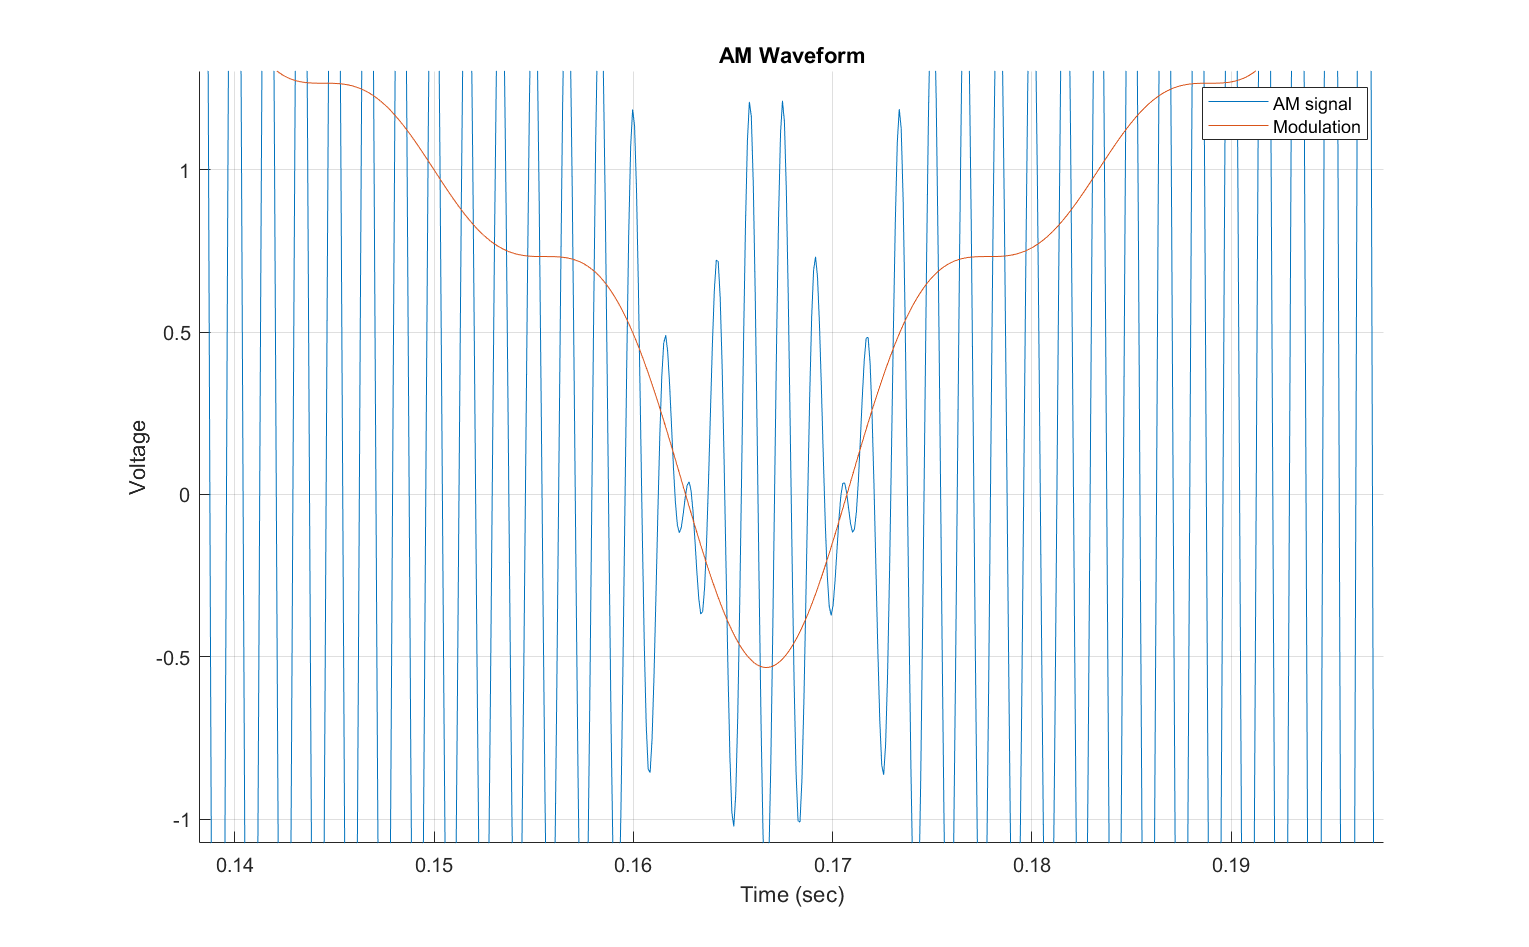
\includegraphics[width=0.5\textwidth]{Images/AM_RX_1/Triangular Wave/Zoomed.png}
            \caption{Detailed view of AM and triangular modulated signal, indicating absence of distortion}
            \label{fig:zoomed-triangle}
        \end{figure}
        

        \section{Demodulation/detection}

        \subsection{AM Detection}
        The script "AM\_RX\_1.m" was configured as per lab guidelines, with waveform fidelity closely mirroring input modulations. Notably, no distortion, clipping, or overmodulation was observed. The signal $o_S$ exhibited a significantly higher amplitude due to carrier multiplication during modulation, with all signals maintaining phase coherence.
        
        \begin{figure}[htbp]
        \centering

        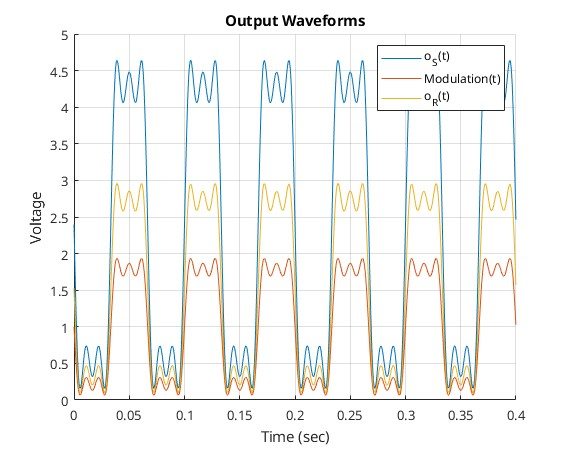
\includegraphics[width=0.5\textwidth]{Images/AM_RX_1/Square Wave/Output Waveforms.jpg}
        \caption{RX outputs comparison}

        \end{figure}

        \begin{figure}[htbp]
        \centering

        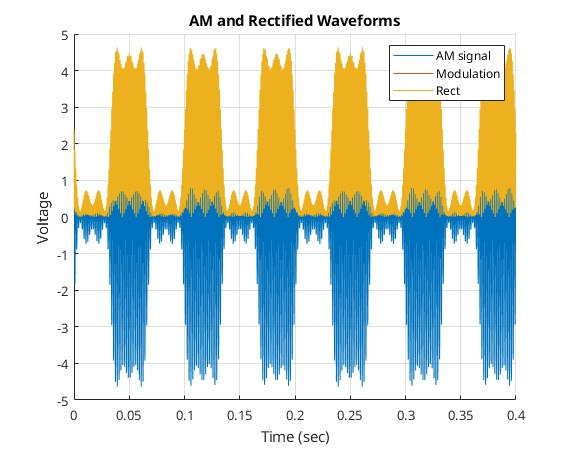
\includegraphics[width=0.5\textwidth]{Images/AM_RX_1/Square Wave/AM and Rectified Waveforms.jpg}
        \caption{AM and rectified waveform}

        \end{figure}

        \newpage

        The waveform parameters were then changed to modulate using a triangle wave approximation. Almost identical behaviour is observed with no distortion or clipping or phase shifts. However there is one key difference - the effects of rectification are clearly seen on the $o_R$ signal. We can see the negative components being mirrored into the positive half (Figure 8).

        \begin{figure}[htbp]
        \centering

        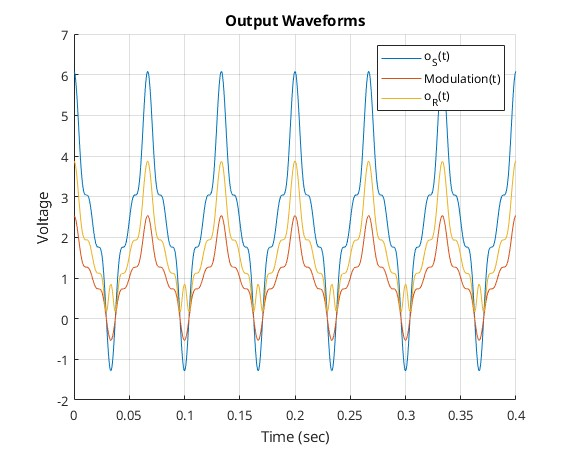
\includegraphics[width=0.5\textwidth]{Images/AM_RX_1/Triangular Wave/Output Waveforms.jpg}
        \caption{RX output comparison for triangle modulation}

        \end{figure}

        \newpage



        \subsection*{Phase Offset in Receiver Carrier}
        Incremental adjustments to the receiver carrier's phase (in $\pi/4$ increments) revealed amplitude variations in the demodulated signal, notably a downshift in $o_s$ by up to -6V and a reduction in $o_R$'s peak-to-peak amplitude. These effects stem from the phase mismatch between transmission and reception carriers, leading to amplitude modulation and phase shifts.        

        \begin{figure}[htbp]
        \centering

        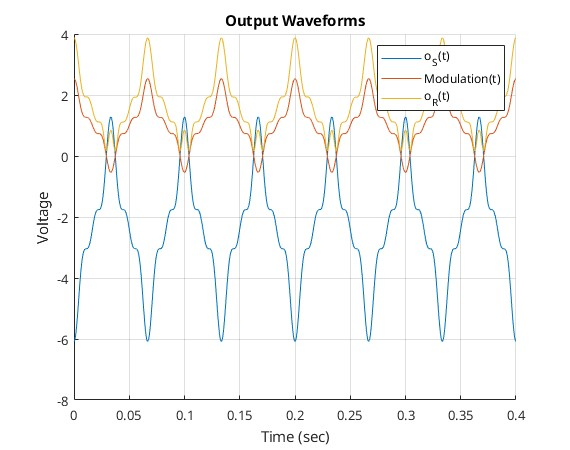
\includegraphics[width=0.5\textwidth]{Images/AM_RX_1/Triangular Wave/Receiver Carrier Phase Offset/Output Waveforms + 4pi 4.jpg}
        \caption{Triangle wave demodulated with receiver carrier phase offset to $4\pi$ }

        \end{figure}

        These changes appear due to the mismatch in phase of the sender and receiver carrier which results in destructive , reducing and shifting the amplitude.


        \subsection*{Frequency Offset in Receiver Carrier}
        Setting the modulation and carrier signals' parameters as specified, it was observed that while $o_R$ demodulated correctly without distortion, $o_S$ was adversely affected. This discrepancy arises from the dependence of $o_S$ on the precise frequency alignment of the carrier and receiver carriers, highlighting the importance of frequency synchronization for accurate demodulation.
        
        \begin{figure}[htbp]
        \centering

        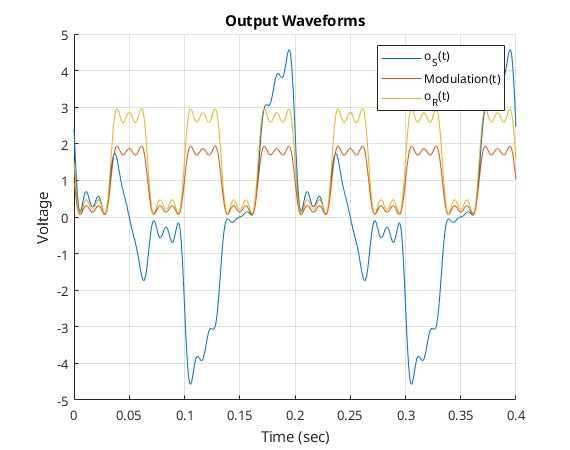
\includegraphics[width=0.5\textwidth]{Images/AM_RX_1/Square Wave/Receiver Carrier Frequency Offset/Output Waveforms.jpg}
        \caption{Square wave with mismatched TX and RX frequencies }

        \end{figure}


        \section{Orthogonal Frequency Division Multiplexing (OFDM)}
        \subsection{OFDM Baseband Signal}
        The parameters in the provided Matlab script were set as per the lab script.
        The following values were calculated:
        \subsection*{"S" Symbol @ 1V}
        \begin{itemize}
            \item ${PEP}$: 41.44W
            \item ${PAPR}$: 8.22
        \end{itemize}

        \subsection*{"S" Symbol @ 2.5V}
        \begin{itemize}
            \item ${PEP}$: 1.8W
            \item ${PAPR}$fair: 8.22
        \end{itemize}

        \subsection{64-QAM on OFDM}
        Matlab was used to calculate PEP and PAPR for each of the following symbols:

        \begin{tabular}{|l|l|l|}
        \hline
        \textbf{Symbols} & \textbf{PEP} & \textbf{PAPR} \\ \hline
        "X" & 141W & 2 \\ \hline
        "+" & 150W & 3.99 \\ \hline
        "Y" & 425W & 3.99 \\ \hline
        "\textless" & 11.4W & 3.97 \\ \hline
        "3" & 57.4W & 3.98 \\ \hline
        "X+Y\textless3" & 1372W & 5.92 \\ \hline
        \end{tabular} \\

        \section{Summary and Comments}
        AM modulation relies on envelope detection, which is susceptible to noise and distortion. In contrast, OFDM signals benefit from coherent detection schemes, offering superior performance in complex multipath environments and effectively mitigating inter-symbol interference, thus presenting a more robust alternative to the traditional AM demodulation techniques.
        
        \end{document}
